\documentclass[a4paper, 12pt]{article}
\usepackage[top=1cm, bottom = 2cm, left = 2cm, right = 2cm]{geometry}
\usepackage[utf8]{inputenc}
\usepackage[brazil]{babel}
\usepackage{listings}
\usepackage[framed, numbered]{matlab-prettifier}
\usepackage[T1]{fontenc}
\usepackage{indentfirst}
\usepackage{graphicx}
\usepackage{epstopdf}
\usepackage{float}
\usepackage{amsmath}
\usepackage{amssymb}
\usepackage{systeme}

\title{Exercício 2 - Aula 4 \\ EET-01}

\author{
  Igor Caldeira Magalhães\\igorcmag@gmail.com
}
\date{08 de maio de 2020}

\begin{document}
\maketitle
\section{Enunciado}

Represente graficamente (matlab ou octave) $x[n]$ e $X(e^{jw})$ para os Exemplos 1 e 2 apresentados em aula.

%O exercício deve ser entregue: Documento simples deve ser apresentado, contendo o seguinte conteúdo:
%Nome da disciplina;
%Nome do aluno;
%Enunciado do exercício;
%Figuras obtidas - Com breve descrição: A Figura xx mostra ...
%Código .m e breve descrição do código matlab (octave);

\section{Solução}

\lstinputlisting[style=Matlab-editor, caption={Código em MATLAB para gerar as sequências exponenciais, exponenciais complexas e suas transformadas de Fourrier, bem como seus gráficos.}, basicstyle = \mlttfamily\scriptsize]{ex2.m}

\begin{figure}[H]
	\centering
	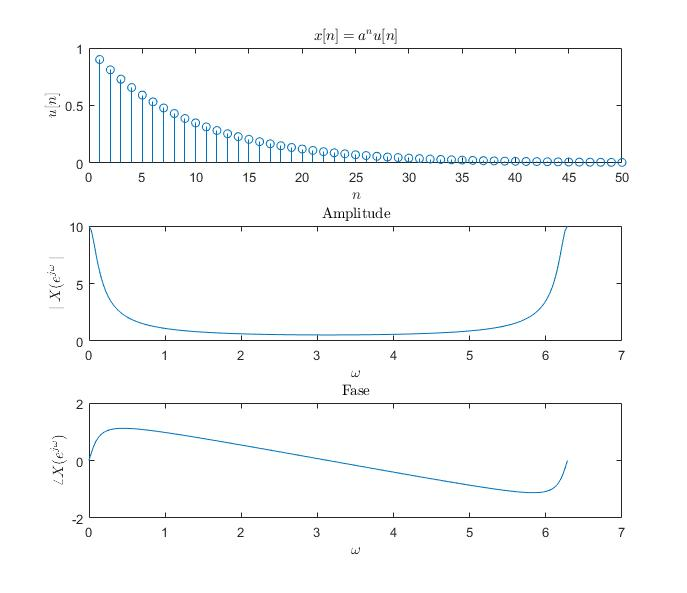
\includegraphics[scale=0.7]{img2.jpg} 
	\caption{Gráficos de $x[n]=a^nu[n]$ e sua transformada de Fourrier. Utilizou-se $a=0.9$.}
	\label{fig:1a}
\end{figure}

\begin{figure}[H]
	\centering
	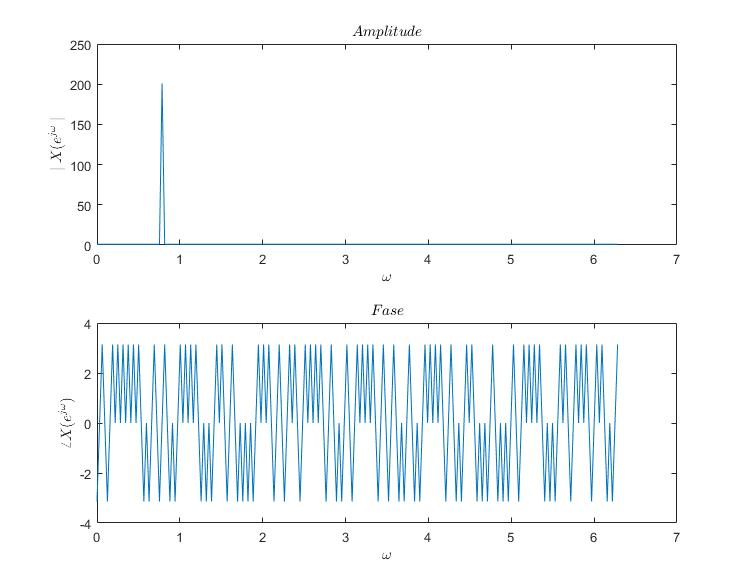
\includegraphics[scale=0.7]{img1.jpg} 
	\caption{Gráficos da transformada de fourrier de  $x[n]=e^{j\omega_0 n}$, definida entre -100 e 100 e com $\omega_0=\pi/4$.}
	\label{fig:1a}
\end{figure}

\end{document}